\begin{exercise}{Sismographe}{2}{Sup}
{Mécanique,Oscillateur harmonique amorti,Ressort,Amortisseur,Oscillateur harmonique forcé}{bermudez,mines}

\begin{questions}
    \questioncours Analogie formelle entre le circuit RLC et le système masse--ressort--amortisseur en régime sinusoïdal forcé. \textsl{On fera un tableau comparant les différentes grandeurs typiques (résonance, facteur de qualité) de ces systèmes du second ordre.}
\end{questions}

\begin{multicols}{2}
    On considère un capteur d'amplitude constitué d'un support et d'une masse $m$ reliés par un ressort de raideur $k$ et de longueur à vide $\ell_0$, et un amortisseur de constante $h$, tout deux de masses négligeables.

    Le support est animé d'un mouvement de type sinusoïdal : $x_1 = b \cos\omega t$ par rapport au référentiel terrestre $(Oxy)$, supposé galiléen.

    \vspace{1cm}

    ~

\begin{figure}[H]
    \centering
    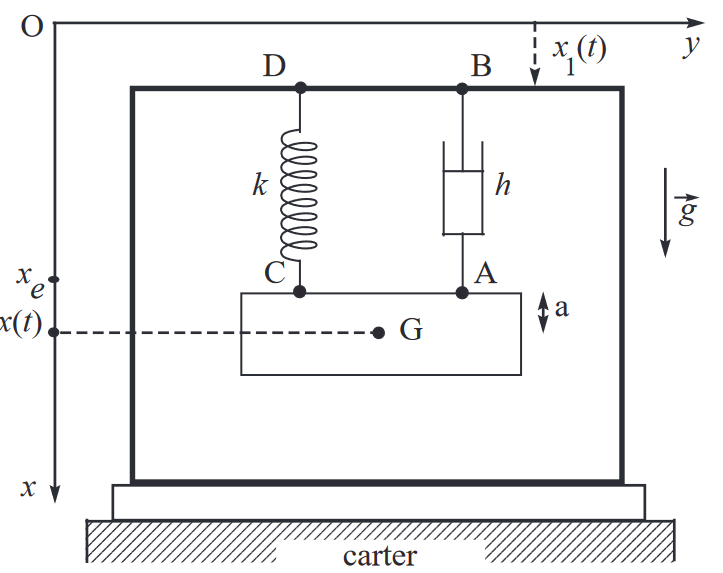
\includegraphics[width=\linewidth]{meca/oscharm/sismo.png}
    \caption{Schéma simplifié du sismomètre.}
\end{figure}
\end{multicols}

\begin{questions}    
\stepcounter{question}
    \question Déterminer l'expression de la position de la masse $m$ à l'équilibre $x_\text{eq}$ quand $x_1(t) = 0$ est immobile.
    \uplevel{On note $X(t) = x(t) - x_1(t) - x_\text{eq}$ la position relative d'une aiguille qui enregistre le signal dans le référentiel du support.}
    \question Déterminer l'équation du mouvement $x(t)$ de la masse $m$ dans le référentiel $(Oxy)$, puis dans la boite $X(t)$.
    \question Comment paramétrer $m$, $\gamma$ et $k$ pour avoir un bon sismomètre ?
\end{questions}
\end{exercise}

\begin{solution}
\begin{questions}
    \questioncours Les deux systèmes se mettent sous la forme :
    $$\ddot{X} + \dfrac{\omega_0}{Q}\dot{X} + \omega_0^2 X = F,$$
    avec : \\
    \begin{tabular}{c|c}
        \textbf{RLC série} & \textbf{Osc. méca} \\ \hline
        $X(t) = u_C(t)$ & $X(t) = x(t)$ \\
        $\omega_0 = \dfrac{1}{\sqrt{LC}}$ & $\omega_0 = \sqrt{\dfrac{k}{m}}$ \\
        $Q = \dfrac{1}{R}\sqrt{\dfrac{L}{C}}$ & $Q = \dfrac{1}{h}\sqrt{mk}$ \\ \hline
        $L$ & $m$ \\
        $C$ & $1/k$ \\
        $R$ & $h$
    \end{tabular}
    \question $x_e = \ell_0 + \dfrac{mg}{k} + a$
    \question PFD dans $(Oxy)$
    $$m\ddot{x} = - h\qty(\dot{x}(t) - \dot{x}_1(t)) - k\qty(x(t) - x_1(t) - x_\text{eq})$$
    ce qui donne
    $$\ddot{X} + \dfrac{\omega_0}{Q}\dot{X} + \omega_0^2 X = F,$$
    avec $F = b\omega^2$.
    \question L'amplitude de réaction est donc donnée par la fonction de transfert :
    $$H = \dfrac{X(t)}{x_1(t)} = \dfrac{1}{\sqrt{\qty(1-\dfrac{\omega_0^2}{\omega^2})^2 + \qty(\dfrac{\omega_0}{Q\omega})^2}}$$
    qui est un passe haut d'ordre 2.

    Ainsi pour limiter l'interie il faut $Q \leqslant 1$ et $\omega_0 \ll \omega_\text{typique séisme}$
\end{questions}
\end{solution}
